\chapter{Future Work} \label{fw}

The future work for this PhD will look at different techniques to finding stopping points. Specifically we will focus on text processing approaches to stopping.



An area that could be further expanded on is the use of using the similarity score in the initial rankings as a basis for comparing documents. In novel work section \ref{simScoreMethod} we examined a technique that uses the top document as the origin point for comparing subsequent documents. To improve the accuracy of the origin point we could try using different points and taking average over a set of points:


\begin{figure}[H]
\center
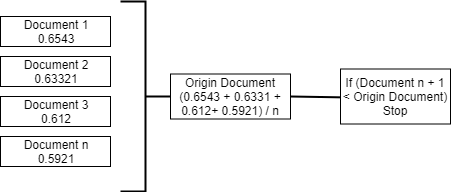
\includegraphics[height=4cm]{figures/originMethod.png}
\caption{Calculating Origin Average}
\end{figure}

The \% difference between document $n+1$ and the origin document would still be used to derive the stopping point.

This approach has the advantage of taking into consideration variability in the quality of the rankings. It also has the advantage of being entirely unsupervised and does not require us to sample the initial document collection. 

A further development of this method is to create an origin document using the document text content itself:

\begin{figure}[H]
\center
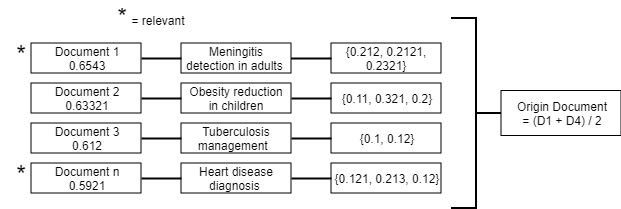
\includegraphics[height=4cm]{figures/origin2.png}
\caption{Generating Origin vector using document content}
\end{figure}

Here we have a further development in that we are using the top $n$ documents to calculate an average document vector by using the content of the document. We can then use vector similarity comparisons such as euclidean distance and cosine similarity to compare the origin document vector to further documents down the rankings.

This method can be tweaked and optimized by standard by applying standard text processing/NLP techniques:

\begin{itemize}
  \item Using Word2Vec to represent abstract features
  \item Language modelling abstract features, trying out different NGram sizes
  \item Pre-processing of a abstracts
  
\end{itemize}

Another method to stopping that could be applied is implementing a classifier. We would still look to use the abstracts as training data for relevant and non-relevant documents. This method would assume we take a sample set of documents as our training data. This training data would then be used to build a classifier to determine if the rest of the documents are relevant or non relevant. We can infer the expected number of relevant documents from the sample and make the assumptions about how many we would need to find to attain a reliability score of 95\%.



\section{Gnatt Chart}

\begin{sidewaysfigure}


\begin{figure}[H]
\center
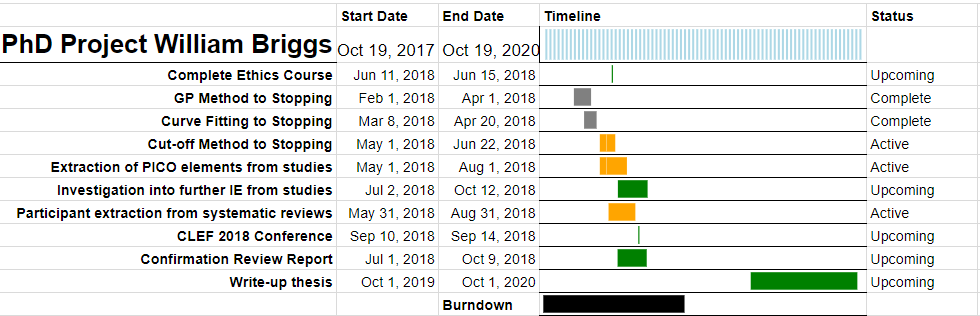
\includegraphics[height=7cm]{figures/gnatt.png}
\caption{Gnatt Chart}
\end{figure}
\end{sidewaysfigure}


